% Fig. 1: shared-embedding multiple access with a fixed pretrained
% codebook and a set of low-dimensional masks (standalone TikZ source of
% fig/fig1_pm.pdf). Compile with  latexmk -pdf fig1_pm.tex , or add
% -outdir=out to keep the byproducts apart and copy out/fig1_pm.pdf to fig/.
\documentclass[tikz,border=2pt]{standalone}
\usepackage{amsmath,amssymb,bm}
\usetikzlibrary{arrows.meta,positioning,calc,fit,decorations.pathreplacing}
\begin{document}
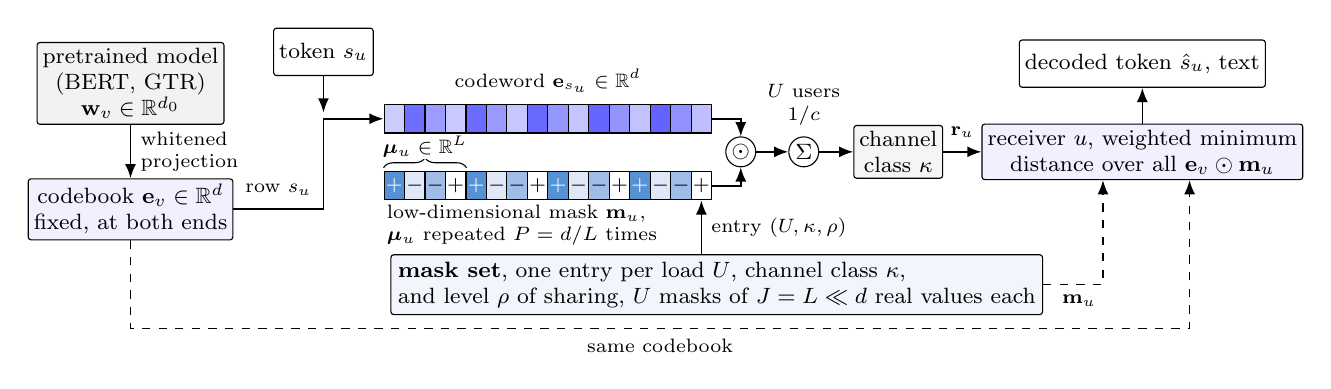
\begin{tikzpicture}[
  font=\footnotesize,
  ar/.style={-{Latex[length=1.8mm,width=1.4mm]},line width=0.6pt},
  blk/.style={draw,rounded corners=1pt,minimum height=6mm,inner sep=2pt,align=center},
  cell/.style={draw,minimum width=2.6mm,minimum height=3.6mm,inner sep=0pt},
  op/.style={draw,circle,inner sep=0.5pt,minimum size=3.8mm},
  brc/.style={decorate,decoration={brace,amplitude=1.3mm}}
]
% ---------------- pretrained model and fixed codebook ----------------
\node[blk,fill=gray!10] (W) at (0,1.05)
  {pretrained model\\(BERT, GTR)\\$\mathbf{w}_v\in\mathbb{R}^{d_0}$};
\node[blk,fill=blue!6] (E) at (0,-0.55)
  {codebook $\mathbf{e}_v\in\mathbb{R}^{d}$\\fixed, at both ends};
\draw[ar] (W.south) -- node[right,font=\scriptsize,align=left] {whitened\\projection} (E.north);

% ---------------- token selects a codeword ----------------
\node[blk] (s) at (2.45,1.45) {token $s_u$};
\foreach \k in {0,...,15}{
  \pgfmathsetmacro{\shade}{20+mod(\k*37,55)}
  \node[cell,fill=blue!\shade] (c\k) at (3.35+0.26*\k,0.6) {};
}
\draw[ar] (E.east) -- (2.45,-0.55) -- (2.45,0.6) -- (c0.west);
\draw[ar] (s.south) -- (2.45,0.68);
\node[font=\scriptsize,anchor=east] at (2.42,-0.30) {row $s_u$};
\node[font=\scriptsize,anchor=south] at ($(c7.north)!0.5!(c8.north)+(0,0.02)$) {codeword $\mathbf{e}_{s_u}\in\mathbb{R}^{d}$};

% ---------------- low-dimensional mask (static entry) ----------------
\foreach \k in {0,...,15}{
  \pgfmathtruncatemacro{\l}{mod(\k,4)}
  \ifcase\l \def\col{cyan!55!blue!70}\def\sg{\color{white}$+$}\or \def\col{cyan!55!blue!12}\def\sg{$-$}\or \def\col{cyan!55!blue!38}\def\sg{$-$}\or \def\col{white}\def\sg{$+$}\fi
  \node[cell,fill=\col,font=\scriptsize] (m\k) at (3.35+0.26*\k,-0.25) {\sg};
}
\draw[brc] ($(m0.north west)+(0,0.04)$) -- node[above=1.1mm,font=\scriptsize,fill=white,inner sep=0.4pt] {$\bm{\mu}_u\in\mathbb{R}^{L}$} ($(m3.north east)+(0,0.04)$);
\node[font=\scriptsize,anchor=north west,align=left,inner sep=1pt] at ($(m0.south west)+(0,-0.02)$)
  {low-dimensional mask $\mathbf{m}_u$,\\$\bm{\mu}_u$ repeated $P=d/L$ times};

% ---------------- superposition, channel, receiver ----------------
\node[op] (mul) at (7.75,0.18) {$\odot$};
\draw[ar] (c15.east) -| (mul.north);
\draw[ar] (m15.east) -| (mul.south);
\node[op] (sum) at (8.55,0.18) {$\Sigma$};
\draw[ar] (mul.east) -- (sum.west);
\node[font=\scriptsize,anchor=south,align=center] at ($(sum.north)+(0,0.02)$) {$U$ users\\$1/c$};
\node[blk,fill=gray!8] (ch) at (9.75,0.18) {channel\\class $\kappa$};
\draw[ar] (sum.east) -- (ch.west);
\node[blk,fill=blue!6] (rx) at (12.85,0.18)
  {receiver $u$, weighted minimum\\distance over all $\mathbf{e}_v\odot\mathbf{m}_u$};
\draw[ar] (ch.east) -- node[above=0.5mm,font=\scriptsize] {$\mathbf{r}_u$} (rx.west);
\node[blk] (txt) at (12.85,1.3) {decoded token $\hat s_u$, text};
\draw[ar] (rx.north) -- (txt.south);

% ---------------- mask set -----------------
\node[draw,fill=cyan!55!blue!5,rounded corners=1pt,inner sep=2.5pt,align=left,anchor=north west] (mset) at (3.3,-1.12)
  {\textbf{mask set}, one entry per load $U$, channel class $\kappa$,\\
   and level $\rho$ of sharing, $U$ masks of $J=L\ll d$ real values each};
% the entry selected by (U, kappa, rho) IS the mask: the arrow ends on the
% mask row (its last cell), not on the wire from the mask to the multiplier
\draw[ar] (m15.south |- mset.north) -- node[right,font=\scriptsize] {entry $(U,\kappa,\rho)$} (m15.south);
\draw[ar,dashed] (mset.east) -| node[pos=0.3,below,font=\scriptsize] {$\mathbf{m}_u$} ($(rx.south)+(-0.5,0)$);
\draw[ar,dashed] ($(E.south)$) -- ++(0,-1.12) -| node[pos=0.25,below,font=\scriptsize] {same codebook} ($(rx.south)+(0.6,0)$);
\end{tikzpicture}
\end{document}
